
\documentclass[letterpaper, reqno,11pt]{article}
\usepackage[margin=1.0in]{geometry}
\usepackage{color,latexsym,amsmath,amssymb}
\usepackage{fancyhdr}
\usepackage{amsthm}
\usepackage{mathtools}
\usepackage{tikz}
\usepackage{float}
\usepackage{centernot}
\usepackage{subcaption}
\usepackage{extarrows}
\usetikzlibrary{hobby}
\usetikzlibrary{shapes.multipart}
\usepackage{pgfplots}
\pgfplotsset{compat=1.7}
\usetikzlibrary{arrows.meta}
\usepackage{cancel}
\usetikzlibrary{decorations.markings}
\usetikzlibrary{shapes}
\usetikzlibrary{arrows}
\usepgfplotslibrary{fillbetween}
\usetikzlibrary{patterns}

\newcommand{\RR}{\mathbb{R}}
\newcommand{\CC}{\mathbb{C}}
\newcommand{\ZZ}{\mathbb{Z}}
\newcommand{\QQ}{\mathbb{Q}}
\newcommand{\NN}{\mathbb{N}}
\DeclareMathOperator{\id}{id}
\def\upint{\mathchoice%
  {\mkern13mu\overline{\vphantom{\intop}\mkern7mu}\mkern-20mu}%
  {\mkern7mu\overline{\vphantom{\intop}\mkern7mu}\mkern-14mu}%
  {\mkern7mu\overline{\vphantom{\intop}\mkern7mu}\mkern-14mu}%
  {\mkern7mu\overline{\vphantom{\intop}\mkern7mu}\mkern-14mu}%
  \int}
\def\lowint{\mkern3mu\underline{\vphantom{\intop}\mkern7mu}\mkern-10mu\int}
\DeclareMathOperator{\card}{card}
\DeclareMathOperator{\Binomial}{Binomial}
\DeclareMathOperator{\Span}{span}
\DeclareMathOperator{\sgn}{sgn}
\pagestyle{fancy}
\lhead{Math 321 Lecture 28}
\rhead{Yuchong Pan}
\begin{document}
\pagenumbering{arabic}
\title{Math 321 Lecture 28}
\author{Yuchong Pan}
\date{March 18, 2019}
\newtheorem{thm}{Theorem}
\newtheorem{defn}{Definition}
\newtheorem*{remark}{Remark}
\newtheorem{claim}{Claim}
\newtheorem{cor}{Corollary}
\newtheorem{lemma}{Lemma}
\newtheorem{prop}{Proposition}
\newtheorem{fact}{Fact}
\maketitle
%

\section{Inverse and Implicit Function Theorems}

\subsection{Differentiability}

Let $\mathbf f : \RR^n \to \RR^m, m, n \geq 1$.

\noindent {\bf Question:} Where is $\mathbf f$ \emph{differentiable}?

\begin{defn}
  \normalfont Say that $\mathbf f$ is {\bf differentiable} at $\mathbf x_0 \in \RR^n$ if there exists a linear transformation $\underbrace{\mathbf A : \RR^n \to \RR^m}_\text{can be represented as an $m \times n$ matrix}$ such that
  \begin{equation} \label{eq:*} \tag{*}
    \frac{\left\lVert \underbrace{\mathbf f(\overbrace{\mathbf x_0}^{\in \RR^n} + \overbrace{\mathbf h}^{\in \RR^n})}_{\in \RR^m} - \underbrace{\mathbf f(\mathbf x_0)}_{\in \RR^m} - \underbrace{\mathbf A}_{m \times n} \underbrace{\mathbf h}_{n \times 1} \right\rVert}{\lVert \mathbf h \rVert} \xrightarrow{\mathbf h \to \mathbf 0} 0.
  \end{equation}
  Call $A = \mathbf f'(\mathbf x_0)$, the ``{\bf partial derivative} of $\mathbf f$ at $\mathbf x_0$''.
\end{defn}

\noindent {\bf Examples:}
\begin{enumerate}
\item If $m = n = 1$, our standard definition of differentiability says that
  \begin{align*}
    & f'(x) \lim_{h \to 0} \frac{f(x_0 + h) - f(x_0)}{h} \text{ exists} \\
    \Leftrightarrow ~ & \lim_{h \to 0} \left(\frac{f(x_0 + h) - f(x_0)}{h} - f'(x_0)\right) = 0 \\
    \Leftrightarrow ~ & \lim_{h \to 0} \frac{f(x_0 + h) - f(x_0) - f'(x_0) h}{h} = 0 \\
    \Leftrightarrow ~ & \lim_{h \to 0} \left|\frac{f(x_0 + h) - f(x_0) - f'(x_0) h}{h}\right| = 0 && \text{which agrees with Definition \eqref{eq:*}}.
  \end{align*}
\item \noindent {\bf Observation:} If $\mathbf A$ exists, it is unique.

  Suppose there exist $\mathbf A, \mathbf B : \RR^n \to \RR^m$ obeying \eqref{eq:*}.
  \begin{align*}
    \frac{\lVert (\mathbf A - B) \mathbf h \rVert}{\lVert \mathbf h \rVert} &= \frac{1}{\lVert \mathbf h \rVert} \left\lVert \mathbf A \mathbf h - \underbrace{\left(\mathbf f(\mathbf x_0 + \mathbf h) - \mathbf f(\mathbf x_0)\right)} + \underbrace{\left(\mathbf f(\mathbf x_0 + \mathbf h) - \mathbf f(\mathbf x_0)\right)} - \mathbf B \mathbf h \right\rVert \\
    &\leq \frac{\lVert \mathbf f(\mathbf x_0 + \mathbf h) - \mathbf f(\mathbf x_0) - \mathbf A \mathbf h \rVert}{\lVert \mathbf h \rVert} + \frac{\lVert \mathbf f(\mathbf x_0 + \mathbf h) - \mathbf f(\mathbf x_0) - \mathbf A \mathbf h \rVert}{\lVert \mathbf h \rVert} \xrightarrow[\mathbf h \to \mathbf 0]{\text{by \eqref{eq:*}}} 0.
  \end{align*}
  
  \noindent {\bf Hence:}
  \begin{equation} \label{eq:**} \tag{**}
    \lim_{\mathbf h \to \mathbf 0} \frac{\lVert (\mathbf A - \mathbf B) \mathbf h \rVert}{\lVert \mathbf h \rVert} = 0.
  \end{equation}
  
  \noindent {\bf Conclusion:} $\mathbf A = \mathbf B$. (If \emph{not}, then there exists $\mathbf v \in \RR^n$ such that $(\mathbf A - \mathbf B) \mathbf v \neq \mathbf 0$. Choose $\mathbf h = t \mathbf v, t \to 0$. Then,
  \[ \frac{\lVert (\mathbf A - \mathbf B) \mathbf h \rVert}{\lVert \mathbf h \rVert} = \frac{\lVert (\mathbf A - \mathbf B) \mathbf v \rVert}{\lVert \mathbf v \rVert} \neq \mathbf 0 \text{, a contradiction}. \]
\item \noindent {\bf Exercises:}
  \begin{enumerate}
  \item Show that if $\mathbf f : \RR^n \to \RR^m$ is \emph{differentiable} at $\mathbf x_0$, then for every $1 \leq j \leq n$,
    \[ \lim_{t \to 0} \frac{\mathbf f(\mathbf x_0 + t \mathbf e_j) - \mathbf f(\mathbf x_0)}{t} = \underbrace{\frac{\partial \mathbf f}{\partial \mathbf x_j} (\mathbf x_0)}_\text{$m$-dimensional vectors} \text{ exists}, \]
    called the $j^\text{th}$ {\bf partial derivative} of $\mathbf f$ at $\mathbf x_0$, where
    \[ \mathbf e_j =
    \begin{pmatrix}
      0 \\
      \vdots \\
      0 \\
      1 \\
      0 \\
      \vdots \\
      0
    \end{pmatrix}
    \text{$\rightarrow$ the $j^\text{th}$ entry}. \]
  \item Show:
    \[ \underbrace{\mathbf A}_{m \times n} =
    \begin{pmatrix}
      \frac{\partial \mathbf f}{\partial x_1}(\mathbf x_0) && \frac{\partial \mathbf f}{\partial x_2}(\mathbf x_0) && \ldots && \frac{\partial \mathbf f}{\partial x_n}(\mathbf x_0)
    \end{pmatrix}
    . \]
  \item However, the converse need not be true. Show that there exists $\mathbf f : \RR^n \to \RR, n \geq 2$ such that all partial derivatives of $\mathbf f$ exists at $\mathbf 0$, but $\mathbf f$ is not differentiable at $\mathbf 0$.
  \end{enumerate}
\end{enumerate}

\subsection{Inverse Function Theorem}

\begin{thm}
  \normalfont Let $\mathbf f : \RR^n \to \RR^n$. Let $E \overset{\text{open}}{\subseteq} \RR^n$ and $\mathbf a \in E$. Assume that $\mathbf f \in C^1(E)$ (i.e., $\underbrace{x}_{\in E} \mapsto \mathbf f'(x)$ is continuous) and $\underbrace{\text{$\overbrace{\mathbf f'(\mathbf a)}^{n \times n}$ is invertible}}_\text{sufficient but not necessary, as the example $h$ shows}$. Set $\mathbf b = \mathbf f(\mathbf a)$.
  \begin{enumerate}
  \item We can invert $\mathbf f$ \emph{locally}: There exists $U \overset{\text{open}}{\subseteq} E \subseteq \RR^n$, $\mathbf b \in V \overset{\text{open}}{\subseteq} \RR^n$ and $\underbrace{g}_{= f^{-1}} : V \xrightarrow[\text{onto}]{\text{$1$-$1$}} U$ such that $f \circ g = \id$ and $g \circ f = \id$.

    \begin{figure}[H]
      \centering
      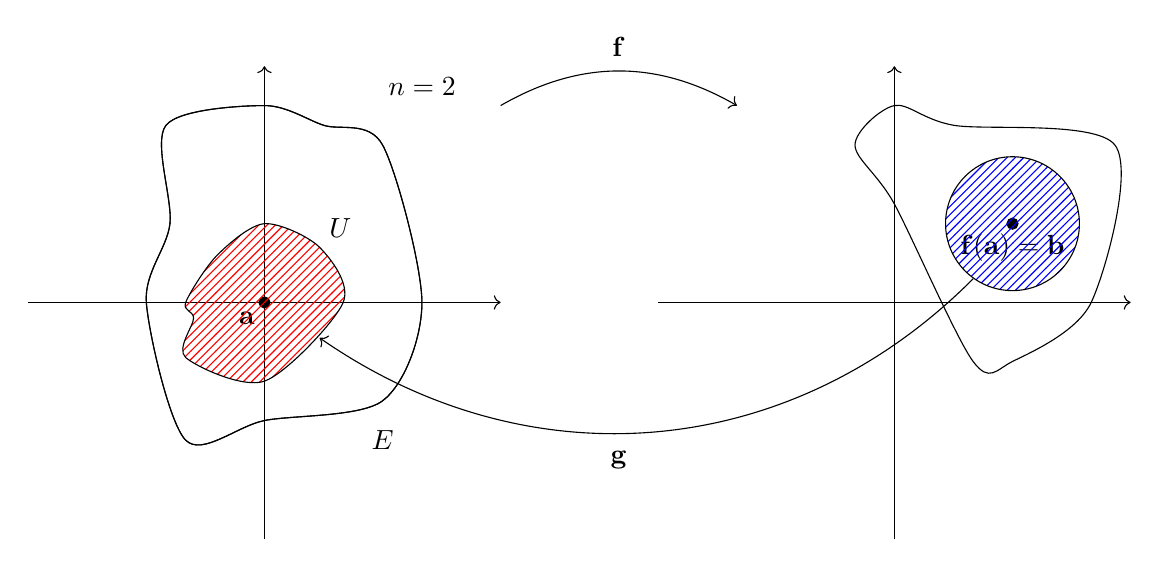
\begin{tikzpicture}
        \draw[->] (0, 0) -- (6, 0);
        \draw[->] (3, -3) -- (3, 3);
        \draw[fill=black] (3, 0) circle (2pt) node[below left] {$\mathbf a$};
        \draw[pattern=north east lines, pattern color=red] plot [mark=none, smooth cycle] coordinates {(4, 0) (3.7, 0.7) (3, 1) (2.4, 0.6) (2, 0) (2.1, -0.2) (2, -0.7) (3, -1)};
        \node[above right] at (3.7, 0.7) {$U$};
        \draw plot [mark=none, smooth cycle] coordinates {(5, 0) (4.5, 2) (3.75, 2.25) (3, 2.5) (1.75, 2.25) (1.8, 1) (1.5, 0) (2, -1.75) (3, -1.5) (4.5, -1.25)};
        \node[below] at (4.5, -1.5) {$E$};
        \node[above] at (5, 2.5) {$n = 2$};
        \draw[->] (8, 0) -- (14, 0);
        \draw[->] (11, -3) -- (11, 3);
        \draw[fill=black] (12.5, 1) circle (2pt) node[below] {$\mathbf f(\mathbf a) = \mathbf b$};
        \draw[pattern=north east lines, pattern color=blue] (12.5, 1) circle (0.85);
        \draw plot [mark=none, smooth cycle] coordinates {(5, 0) (4.5, 2) (3.75, 2.25) (3, 2.5) (1.75, 2.25) (1.8, 1) (1.5, 0) (2, -1.75) (3, -1.5) (4.5, -1.25)};
        \draw plot [mark=none, smooth cycle] coordinates {(13.5, 0) (13.8, 2) (11.75, 2.25) (11, 2.5) (10.5, 2) (11, 1.25) (12, -0.75) (12.5, -0.75)};
        \draw[->] (6, 2.5) to[bend left] (9, 2.5);
        \node at (7.5, 3.25) {$\mathbf f$};
        \draw[->] (12, 0.3) to[bend left=40] (3.7, -0.45);
        \node at (7.5, -2) {$\mathbf g$};
      \end{tikzpicture}
    \end{figure}

    \begin{align*}
      \mathbf g \circ \mathbf f(\mathbf u) &= \mathbf u \qquad \forall \mathbf u \in U, \\
      \mathbf f \circ \mathbf g(\mathbf v) &= \mathbf v \qquad \forall \mathbf v \in V.
    \end{align*}
  \item $g \in C^1(V)$.
  \end{enumerate}

  \noindent {\bf Example:} Suppose $n = 1$. Then $f'(a)$ invertible means that $f'(a) \neq 0$. Let $f(x) = x^2, x \in (-a, a)$. Then $f'(0) = 0$ and $f$ is not invertible in any neighborhood of the origin.

  \begin{figure}[H]
    \centering
    \begin{tikzpicture}[
        declare function={f(\x)=\x*\x;},
      ]
      \begin{axis}[
          xmin=-2,
          xmax=2,
          ymin=-1,
          ymax=4,
          xtick={-1.6, 1.6},
          xticklabels={$-a$, $a$},
          ymajorticks=false,
          axis x line=center,
          axis y line=center,
          clip=false,
        ]
        \addplot[thick, blue, domain={-1.8:1.8}](x,{f(x)}) node [above right] {$y = x^2$};
        \draw[dashed] (axis cs:-1.6, 0) -- (axis cs:-1.6, {f(-1.6)});
        \draw[dashed] (axis cs:1.6, 0) -- (axis cs:1.6, {f(1.6)});
        \draw[thick, red] (axis cs:-1.8, 1) -- (axis cs:1.8, 1);
        \draw[dashed, red] (axis cs:-1, 0) -- (axis cs:-1, 1);
        \draw[dashed, red] (axis cs:1, 0) -- (axis cs:1, 1);
      \end{axis}
    \end{tikzpicture}
  \end{figure}

  Let $h(x) = x^3$. Then $h'(0) = 0$. However, $h$ is invertible near $0$.

  \begin{figure}[H]
    \centering
    \begin{tikzpicture}[
        declare function={h(\x)=\x*\x*\x;},
      ]
      \begin{axis}[
          xmin=-2,
          xmax=2,
          ymin=-6,
          ymax=6,
          xmajorticks=false,
          ymajorticks=false,
          axis x line=center,
          axis y line=center,
          clip=false,
        ]
        \addplot[thick, blue, domain={-1.8:1.8}](x,{h(x)}) node [above right] {$y = x^3 = h(x)$};
      \end{axis}
    \end{tikzpicture}
  \end{figure}
\end{thm}

\end{document}
